% =====================================================================
% AVS Quantum Science submission
% Manuscript: GHZ-Based Quantum Secret Sharing
% Target journal: AVS Quantum Science
% =====================================================================

\documentclass[aip,amsmath,amssymb,reprint,longbibliography]{revtex4-2}
\pdfoutput=1

% ---------------------------------------------------------------------
% Packages
% ---------------------------------------------------------------------
\usepackage[utf8]{inputenc}
\usepackage[T1]{fontenc}
\usepackage[english]{babel}
\usepackage{amsmath,amssymb,amsfonts}
\usepackage{mathtools}
\usepackage{amsthm}
\usepackage{bm}
\usepackage{braket}
\usepackage{graphicx}
\usepackage{booktabs}
\usepackage{multirow}
\usepackage{siunitx}
\usepackage{float}
\usepackage{xcolor}
\usepackage{hyperref}
\usepackage{cleveref}
\usepackage{enumitem}

% ---------------------------------------------------------------------
% Theorem-like environments
% ---------------------------------------------------------------------
\newtheorem{theorem}{Theorem}
\newtheorem{proposition}{Proposition}
\newtheorem{lemma}{Lemma}
\newtheorem{definition}{Definition}
\newtheorem{corollary}{Corollary}

% ---------------------------------------------------------------------
% Custom commands
% ---------------------------------------------------------------------
\newcommand{\ghz}{\mathrm{GHZ}}
\newcommand{\cnot}{\textsc{cnot}}
\newcommand{\qber}{\mathrm{QBER}}
\newcommand{\fid}{\mathcal{F}}
\newcommand{\Tr}{\operatorname{Tr}}
\newcommand{\cE}{\mathcal{E}}
\newcommand{\cD}{\mathcal{D}}
\newcommand{\ketzero}{\ket{0}^{\otimes n}}
\newcommand{\ketone}{\ket{1}^{\otimes n}}
\newcommand{\brazero}{\bra{0}^{\otimes n}}
\newcommand{\braone}{\bra{1}^{\otimes n}}

% ---------------------------------------------------------------------
% Metadata
% ---------------------------------------------------------------------
\begin{document}

\title{Dual-basis witnesses and hardware noise benchmarks for GHZ quantum secret sharing on superconducting processors}

\author{Tanvir Hassan}
\email{tanvir6307@gmail.com}
\affiliation{Department of Physics, Jagannath University, Dhaka 1100, Bangladesh}

\begin{abstract}
GHZ-based quantum secret sharing offers a compact route to multipartite cryptography, but present superconducting processors expose it to several simultaneous error mechanisms.  This work asks which experimentally accessible signatures remain useful for benchmarking secret reconstruction and diagnosing eavesdropping-like disturbances under realistic device noise.  We combine a dual-basis witness theory with density-matrix and shot-based simulations of an HBB-inspired GHZ secret-sharing primitive, using an eight-channel superconducting-noise model calibrated from IBM Quantum device parameters.  The analysis shows that computational-basis population tests alone can miss which-branch information leakage, whereas adding an $X$-basis coherence check flags both intercept--resend and entangle--measure individual attacks in this diagnostic model.  For three-party sharing, the model gives a GHZ fidelity of $0.950\pm0.002$ and a reconstruction success rate of $89.7\%\pm0.2\%$; up to seven parties, the states remain above the multipartite-entanglement witness threshold.  A first-order channel-resolved error budget identifies SPAM as the leading limitation, accounting for about $67\%$ of the summed three-qubit error penalty.  Hardware validation on IBM Marrakesh gives a root-mean-square simulation--experiment fidelity gap of $1.9\%$ for $n=3,5,7$.  These results define a practical benchmark suite for near-term GHZ secret-sharing experiments; they are intended as device-level diagnostics rather than a composable cryptographic security proof.
\end{abstract}

\maketitle

\section{Introduction}
\label{sec:introduction}

Secret sharing allows a dealer to distribute information among several parties such that authorized coalitions can recover the secret whereas unauthorized subsets cannot.  Classical threshold schemes were introduced by Shamir and Blakley~\cite{Shamir1979,Blakley1979}.  Quantum secret sharing (QSS) strengthens this idea by exploiting entanglement, measurement disturbance, and the no-cloning principle.  The Hillery--Bu\v{z}ek--Berthiaume (HBB) protocol~\cite{Hillery1999} uses a three-party GHZ state to distribute a classical secret whose reconstruction requires collaboration among the parties, while related foundational work established entanglement-based splitting and quantum-threshold secret sharing~\cite{Karlsson1999,Cleve1999,Gottesman2000}.  The natural $n$-party resource is
\begin{equation}
\ket{\ghz_n}=\frac{1}{\sqrt{2}}\left(\ket{0}^{\otimes n}+\ket{1}^{\otimes n}\right).
\label{eq:ghz_state}
\end{equation}
This state was introduced by Greenberger, Horne, and Zeilinger~\cite{Greenberger1989}.
GHZ-state QSS has close connections to multipartite entanglement verification, quantum networks, and device-level benchmarking.

Experiments have demonstrated QSS or related multipartite entanglement on photonic systems~\cite{Chen2005,Schmid2005,Bell2014,Williams2019,Lu2016}, trapped ions~\cite{Monz2011}, and superconducting qubits~\cite{Mooney2019,Wei2020,Song2019}.  Related GHZ/cat-state benchmarks have also been reported in Rydberg-atom arrays~\cite{Omran2019}.  In parallel, theory has developed graph-state, hierarchical, high-dimensional, communication-efficient, and anonymous-network variants~\cite{Markham2008,Qin2020,Tavakoli2015,Senthoor2019,Lipinska2018}.  For current noisy intermediate-scale quantum devices~\cite{Preskill2018,Bharti2022}, however, a pressing experimental question is not composable security in the ideal cryptographic limit, but which measurable signatures remain reliable as hardware-level benchmarks and attack diagnostics under realistic superconducting noise.

Superconducting transmon processors exhibit a heterogeneous error landscape: relaxation and dephasing~\cite{Krantz2019}, stochastic gate errors~\cite{Magesan2012}, coherent over-rotations~\cite{McKay2017}, residual $ZZ$ crosstalk~\cite{Mundada2019,Malekakhlagh2020}, leakage outside the computational subspace~\cite{Rol2019,Wood2018}, low-frequency flux noise~\cite{Ithier2005,Paladino2014}, collective dephasing~\cite{Clemens2004,Chirolli2008}, and SPAM errors~\cite{Gambetta2007}.  GHZ states are especially sensitive because a single mechanism can affect either the computational-basis populations or the global coherence.  This separation is central to QSS: an adversary can leave $Z$-basis correlations nearly unchanged while destroying the phase coherence that certifies genuine multipartite entanglement.

This paper contributes a hardware-oriented benchmarking and diagnostic framework for noisy GHZ-based QSS, supported by a dual-basis witness theory.  Instead of treating the simulation as the primary result, we identify the two quantities that control both fidelity estimation and individual-attack diagnostics:
\begin{equation}
P_Z=p_{0\cdots0}+p_{1\cdots1},\qquad C_X=|\langle X^{\otimes n}\rangle|.
\label{eq:pz_cx_intro}
\end{equation}
Within the GHZ support, the combination $(P_Z+C_X)/2$ estimates the target-state fidelity, while the separation between $P_Z$ and $C_X$ distinguishes population-preserving disturbances from ordinary population loss.  We prove that entangle--measure attacks can be invisible to $Z$-only monitoring but must be visible in $X$-basis coherence loss.  We then test this diagnostic principle using a calibrated eight-channel model and hardware data.

The main contributions are:
\begin{enumerate}[leftmargin=*]
\item a dual-basis witness theory for noisy GHZ secret-sharing benchmarks, including analytical statements connecting $Z$-basis population, $X$-basis coherence, individual-attack diagnostics, and reconstruction probability;
\item an eight-channel superconducting-noise model parameterized from IBM Quantum calibration data;
\item a channel-resolved error budget showing that SPAM, rather than CNOT error alone, dominates short-depth GHZ-QSS performance;
\item a simulation-to-hardware validation on IBM Marrakesh for $n=3,5,7$.
\end{enumerate}

\section{Dual-basis theory of noisy GHZ secret sharing}
\label{sec:theory}

\subsection{GHZ preparation and fidelity observables}
\label{subsec:ghzprep}

An $n$-qubit GHZ state is prepared on a linear chain using
\begin{equation}
U_{\ghz}^{(n)}=\left(\prod_{k=1}^{n-1}\cnot_{k-1,k}\right)H_0.
\label{eq:ghz_circuit}
\end{equation}
For an arbitrary output state $\rho$, the exact GHZ fidelity is~\cite{NielsenChuang2010}
\begin{align}
\fid(\rho)&=\bra{\ghz_n}\rho\ket{\ghz_n} \\
&=\frac{1}{2}\left(\rho_{0\cdots0,0\cdots0}+\rho_{1\cdots1,1\cdots1}\right)
+\mathrm{Re}\,\rho_{0\cdots0,1\cdots1}.
\label{eq:exact_fidelity}
\end{align}
Experimentally, the population part is estimated in the computational basis as $P_Z=p_{0\cdots0}+p_{1\cdots1}$, while the coherence is bounded by parity measurements in the $X$ basis:
\begin{equation}
C_X=|\langle X^{\otimes n}\rangle|.
\label{eq:cx_def}
\end{equation}
For states whose relevant weight remains in the GHZ subspace, the two-observable estimator is
\begin{equation}
\fid_{ZX}=\frac{P_Z+C_X}{2}.
\label{eq:two_observable_fidelity}
\end{equation}
The witness $\fid_{ZX}>1/2$ certifies genuine multipartite entanglement for the intended GHZ resource~\cite{Guhne2009,Toth2005}.

\subsection{Noisy GHZ secret-sharing benchmark}
\label{subsec:hbb}

The noisy GHZ secret-sharing benchmark considered here has four stages.  First, the dealer prepares and distributes $\rho\approx\ket{\ghz_n}\!\bra{\ghz_n}$.  Second, a random fraction $f_{\rm check}$ of rounds is measured in the $X$ basis to estimate the parity-error rate
\begin{equation}
\qber_X=\Pr\left[\bigoplus_{i=1}^n x_i=1\right].
\label{eq:qberx}
\end{equation}
Third, in data rounds the dealer encodes a bit $s$ by applying the computational-basis bit flip $X^s$ to her qubit.  Fourth, all parties measure in the $Z$ basis and reconstruct using
\begin{equation}
\hat{s}=a\oplus \mathrm{maj}(b_2,\ldots,b_n),
\label{eq:decoder}
\end{equation}
where $a$ is the dealer's outcome and $\mathrm{maj}$ denotes majority voting over the remaining parties.  The use of $X^s$ is essential for this data-round decoder: a phase operation $Z^s$ would leave all computational-basis measurement probabilities unchanged and could not be recovered by Eq.~\eqref{eq:decoder} without complementary-basis data-round measurements.

The diagnostic rule used in the attack simulations is
\begin{equation}
\begin{aligned}
\mathrm{detect}=1
\Longleftrightarrow{}&
\Delta R_Z>\delta_Z\\
&{}\lor\ \qber_X>\eta_{\rm honest}+\delta_X ,
\end{aligned}
\label{eq:detection_rule}
\end{equation}
where $\Delta R_Z$ is the degradation of the $Z$-basis reconstruction success rate.  We use $\delta_Z=0.10$ and $\delta_X=0.05$.  The constants can be tuned to the expected honest-device noise level; their purpose is to separate ordinary calibration noise from attack-induced deviations.

\subsection{Population--coherence separation}
\label{subsec:population_coherence}

The following proposition is the key reason a dual-basis test is necessary.

\begin{proposition}[Population-preserving attacks suppress GHZ coherence]
\label{prop:coherence_suppression}
Let an adversary couple an ancilla to one qubit of the GHZ state such that
\begin{equation}
\begin{aligned}
\ket{0}\ket{e_0}&\mapsto\ket{0}\ket{e_0'},\\
\ket{1}\ket{e_0}&\mapsto\ket{1}\ket{e_1'} ,
\end{aligned}
\label{eq:which_branch_attack}
\end{equation}
while preserving computational-basis populations.  After tracing out Eve, the honest parties hold
\begin{equation}
\begin{aligned}
\rho_E=\frac{1}{2}\Bigl(&\ketzero\!\brazero+\ketone\!\braone\\
&+\gamma\ketzero\!\braone+\gamma^*\ketone\!\brazero\Bigr),
\end{aligned}
\label{eq:rho_eve}
\end{equation}
where $\gamma=\langle e_1'|e_0'\rangle$.  Therefore
\begin{equation}
P_Z=1,
\qquad
C_X=|\gamma|.
\label{eq:pz_cx_gamma}
\end{equation}
In particular, a perfect which-branch attack with $\langle e_1'|e_0'\rangle=0$ is invisible to $Z$-basis population tests but maximally visible in the $X$-basis coherence test.
\end{proposition}

\begin{proof}
Apply the controlled interaction in Eq.~\eqref{eq:which_branch_attack} to Eq.~\eqref{eq:ghz_state} and trace out Eve's ancilla.  The diagonal terms are unchanged, so $P_Z=1$.  The only surviving off-diagonal term is multiplied by the ancilla overlap $\gamma$.  Since $X^{\otimes n}$ exchanges $\ketzero$ and $\ketone$, $\langle X^{\otimes n}\rangle=\mathrm{Re}\,\gamma$ up to a known analysis phase, and the optimized coherence magnitude is $C_X=|\gamma|$.
\end{proof}

\begin{corollary}[Necessity of dual-basis monitoring]
\label{cor:dual_basis}
Any QSS implementation that monitors only $Z$-basis correlations cannot distinguish the ideal GHZ state from the fully dephased mixture
\begin{equation}
\rho_{\rm mix}=\frac{1}{2}\left(\ketzero\!\brazero+\ketone\!\braone\right),
\label{eq:ghz_mixture}
\end{equation}
whereas the $X$-basis witness gives $C_X=0$ for $\rho_{\rm mix}$ and $C_X=1$ for the ideal GHZ state.
\end{corollary}

\subsection{Reconstruction success under independent readout noise}
\label{subsec:majority_theory}

The majority decoder in Eq.~\eqref{eq:decoder} behaves as a classical repetition code on the non-dealer outcomes.  If the relevant bit-flip probability per non-dealer qubit is $p<1/2$, the probability that the majority vote is correct for $m=n-1$ helpers is
\begin{equation}
P_{\rm maj}(m,p)=\sum_{k=0}^{\lfloor (m-1)/2\rfloor}\binom{m}{k}p^k(1-p)^{m-k},
\label{eq:maj_success}
\end{equation}
for odd $m$, with the usual random tie-breaking modification for even $m$.  Thus the reconstruction can remain high even when the full many-body fidelity has decreased, because the operational decoding depends primarily on the marginal bit-error rate, not only on global coherence.

\section{Composite superconducting noise model}
\label{sec:noise_model}

We model the implemented channel as a composition of eight error processes.  Parameters are anchored to IBM Quantum Falcon-class calibration data and literature values, while hardware validation is performed on IBM Marrakesh.  The primary parameter set is summarized in \cref{tab:params}.

\begin{table}[H]
\centering
\caption{Device parameters used in the calibrated noise model.  Values represent representative IBM Quantum Falcon-class parameters used for the primary simulation.}
\label{tab:params}
\small
\resizebox{\columnwidth}{!}{%
\begin{tabular}{@{}lcc@{}}
\toprule
Parameter & Value & Unit \\
\midrule
$T_1$ mean & $105\pm15$ & $\mu$s \\
$T_2$ mean & $116\pm20$ & $\mu$s \\
Single-qubit gate error & $3.8\times10^{-4}$ & -- \\
CNOT gate error & $9.6\times10^{-3}$ & -- \\
Readout error & $2.6\times10^{-2}$ & -- \\
$t_{1Q}$ / $t_{\cnot}$ / $t_m$ & $50/300/2000$ & ns \\
Leakage, $1Q$ / CNOT & $5\times10^{-4}/5\times10^{-3}$ & -- \\
Residual $ZZ$ coupling & $50$ & kHz \\
Over-rotation $\epsilon$ & $10^{-3}$ & rad \\
Dephasing correlation $\xi$ & $0.3$ & -- \\
\bottomrule
\end{tabular}}
\end{table}

Thermal relaxation is implemented using amplitude damping and phase damping after each gate, with
\begin{equation}
\begin{aligned}
p_{T_1}&=1-e^{-t_g/T_1},&
p_\phi&=1-e^{-t_g/T_\phi},\\
T_\phi&=\left(T_2^{-1}-(2T_1)^{-1}\right)^{-1}.
\end{aligned}
\label{eq:t1t2_rates}
\end{equation}
Stochastic gate errors are modeled by one- and two-qubit depolarizing channels with rates $p_1$ and $p_2$.  Coherent calibration errors are represented by small residual rotations $R_z(\pi\epsilon)$.  Residual $ZZ$ coupling is modeled as
\begin{equation}
\begin{aligned}
U_{ZZ}(\theta)&=\exp[-i(\theta/2)Z\otimes Z],\\
\theta&=2\pi\nu_{ZZ}t_{\cnot}.
\end{aligned}
\label{eq:zz_noise}
\end{equation}
Leakage is approximated as a depolarizing loss channel within the computational subspace.  Collective dephasing is included through a correlated phase-damping contribution scaled by $\xi$.  Low-frequency $1/f^\alpha$ noise is incorporated through measured $T_2$ values and included analytically in the error budget.  SPAM noise consists of a thermal preparation bit flip with probability $p_{\rm th}\approx0.02$ and asymmetric readout confusion probabilities $P(1|0)\approx0.01$ and $P(0|1)\lesssim0.05$.

For a CNOT on qubits $(i,j)$ the effective channel is written as
\begin{equation}
\cE_{\cnot}^{(i,j)}=
\cE_{\rm depol}^{(2)}\circ
\cE_{T_1/T_2}\circ
\cE_{\rm leak}\circ
\cE_{ZZ}\circ
\cE_{\rm coh}\circ
\cE_{\rm coll}.
\label{eq:channel_composition}
\end{equation}
A global scale $\lambda$ multiplies all elementary error rates, enabling threshold analysis.

\section{Methods}
\label{sec:methods}

Simulations use Qiskit and Qiskit Aer~\cite{Qiskit2024,Aer2024} with two back ends.  Density-matrix simulation is used for state fidelity and scaling; a first-order analytical decomposition is used for channel-resolved error budgets; shot-based simulation with $8192$ shots is used for secret-sharing statistics, Monte Carlo convergence, and attack detection.  For each $n\in\{3,4,5,6,7\}$ we prepare the GHZ circuit of Eq.~\eqref{eq:ghz_circuit}, apply the composite noise model, and estimate the observables in Eq.~\eqref{eq:pz_cx_intro}.  Protocol trials use the secret bit string ``101'', $f_{\rm check}=0.2$, and majority-vote reconstruction.  Reported uncertainties are standard deviations over $100$ independent trials unless otherwise stated.  Confidence intervals are estimated by bootstrap resampling with $10^4$ resamples.

Attack simulations use two canonical strategies.  In intercept--resend, Eve measures one transmitted qubit and re-prepares the measured state.  In entangle--measure, Eve applies a CNOT from the target qubit to a private ancilla and later measures her ancilla.  The latter is the operational version of the which-branch attack in \cref{prop:coherence_suppression}.

Hardware validation uses linear GHZ preparation circuits on IBM Marrakesh for $n=3,5,7$.  Both $Z$-basis and $X$-basis circuits are executed with $4096$ shots in IBM Quantum job \texttt{d6a62bpd1ejc73c8b6h0}, recorded in the repository metadata with timestamp 2026-02-17T18:38:00, and fidelity is estimated using Eq.~\eqref{eq:two_observable_fidelity}.  The circuits use logical qubits $0,\ldots,n-1$ before transpilation and are transpiled with the backend preset pass manager at optimization level 1; physical layouts are selected by the transpiler rather than fixed manually.  No readout mitigation, zero-noise extrapolation, or other error-mitigation post-processing is applied to the hardware counts.  The comparison is intentionally cross-architectural: the main model uses Falcon-class calibration parameters and standard IBM superconducting-processor error channels~\cite{Gambetta2017}, while validation is performed on a Heron-class processor.  This tests whether the model captures the relevant physical mechanisms rather than merely fitting a single device instance.

\section{Results}
\label{sec:results}

\subsection{GHZ fidelity and scaling}
\label{subsec:fidelity_scaling}

\Cref{tab:fidelity} reports GHZ fidelities under the full composite model.  All states from $n=3$ to $n=7$ remain above the witness threshold $\fid>1/2$.

\begin{table}[H]
\centering
\caption{GHZ fidelity under the full composite noise model.  Uncertainties are standard deviations over $100$ trials; confidence intervals are bootstrap estimates.}
\label{tab:fidelity}
\resizebox{\columnwidth}{!}{%
\begin{tabular}{ccccc}
\toprule
$n$ & $\fid$ & $\sigma_\fid$ & 95\% CI & $\fid>1/2$ \\
\midrule
3 & 0.9504 & 0.0024 & [0.9457, 0.9551] & yes \\
4 & 0.9166 & 0.0031 & [0.9106, 0.9226] & yes \\
5 & 0.8839 & 0.0035 & [0.8770, 0.8908] & yes \\
6 & 0.8688 & 0.0037 & [0.8615, 0.8761] & yes \\
7 & 0.8541 & 0.0039 & [0.8465, 0.8618] & yes \\
\bottomrule
\end{tabular}}
\end{table}

The fidelity decay is well described by
\begin{equation}
\begin{aligned}
\fid(n)&=A e^{-\alpha n}+C,\\
A&=0.357\pm0.041,\\
\alpha&=0.330\pm0.073,\\
C&=0.819\pm0.016,
\end{aligned}
\label{eq:fit_result}
\end{equation}
with $R^2=0.997$.  The nonzero offset reflects the fact that, over this limited size range, dominant SPAM contributions do not scale in the same way as coherent GHZ dephasing or CNOT accumulation.

\begin{figure}[H]
\centering
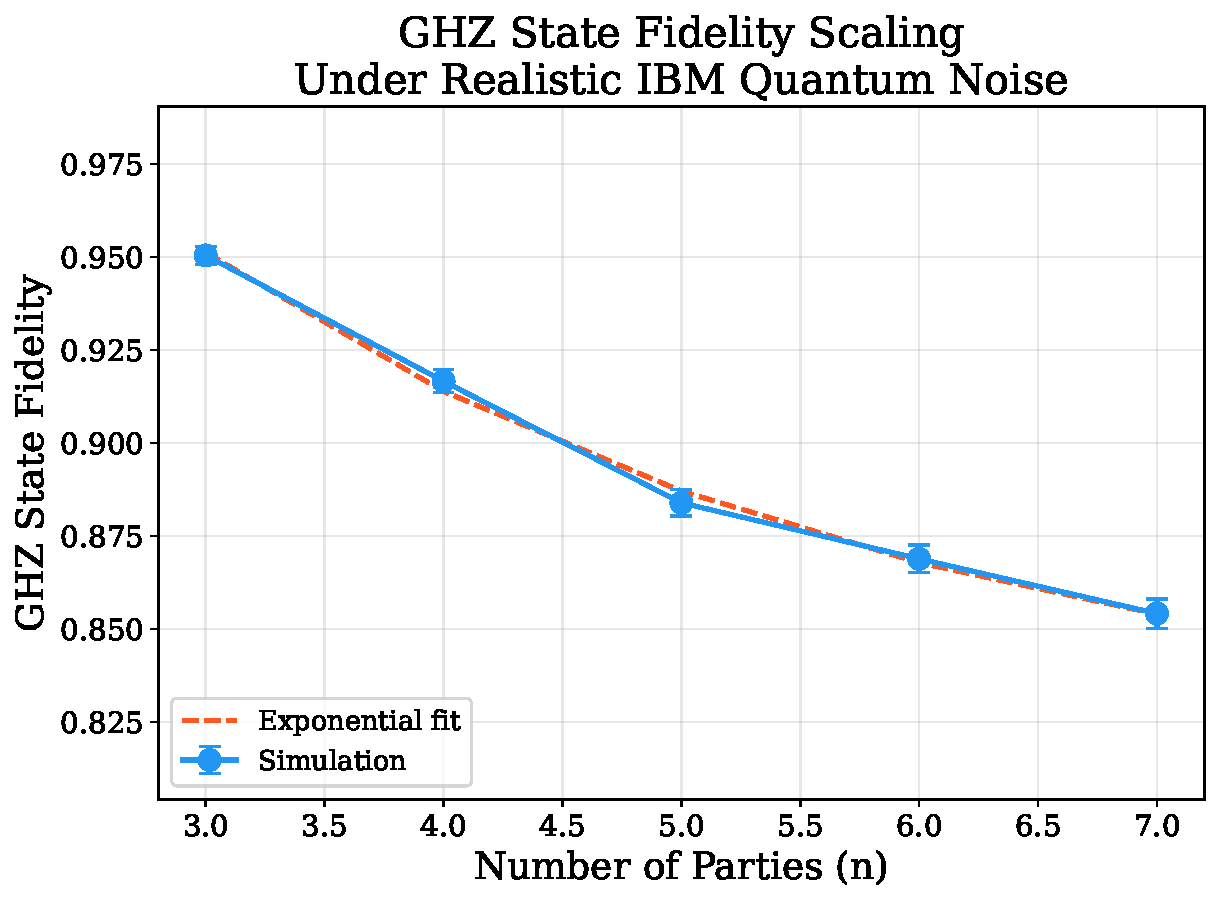
\includegraphics[width=\columnwidth]{figures/fig1_ghz_scaling.pdf}
\caption{GHZ fidelity versus party number with the fit in Eq.~\eqref{eq:fit_result}.  Error bars show bootstrap confidence intervals.}
\label{fig:scaling}
\end{figure}

\subsection{Channel-resolved error budget}
\label{subsec:error_budget}

\Cref{tab:budget} reports a first-order channel penalty budget for the three-qubit experiment.  The entries are independent operational penalties estimated from calibration-scale error rates and should not be interpreted as a normalized decomposition of $1-\fid$ in \cref{tab:fidelity}; in particular, measurement and preparation penalties enter the operational benchmark even though they are not simply additive contributions to the density-matrix state infidelity.  SPAM is the leading contribution in this first-order budget: readout and preparation together account for approximately $67\%$ of the summed penalty.  This implies that optimizing readout, reset, and calibration can improve short-depth GHZ-QSS more efficiently than focusing exclusively on two-qubit gate fidelity.

\begin{table}[H]
\centering
\caption{First-order operational error budget for the three-qubit GHZ benchmark.  The total is a summed penalty estimate, not $1-\fid$ from \cref{tab:fidelity}.}
\label{tab:budget}
\resizebox{\columnwidth}{!}{%
\begin{tabular}{@{}lcc@{}}
\toprule
Error source & Penalty (\%) & Absolute penalty \\
\midrule
Readout errors & 7.77 & 0.0777 \\
State preparation & 6.00 & 0.0600 \\
CNOT depolarizing & 1.90 & 0.0190 \\
$T_1$ relaxation & 1.85 & 0.0185 \\
$T_2$ dephasing & 1.68 & 0.0168 \\
Leakage & 1.05 & 0.0105 \\
$ZZ$ crosstalk & 0.20 & 0.0020 \\
$H$-gate depolarizing & 0.04 & 0.0004 \\
\midrule
Total first-order penalty & 20.49 & 0.2049 \\
\bottomrule
\end{tabular}}
\end{table}

\begin{figure}[H]
\centering
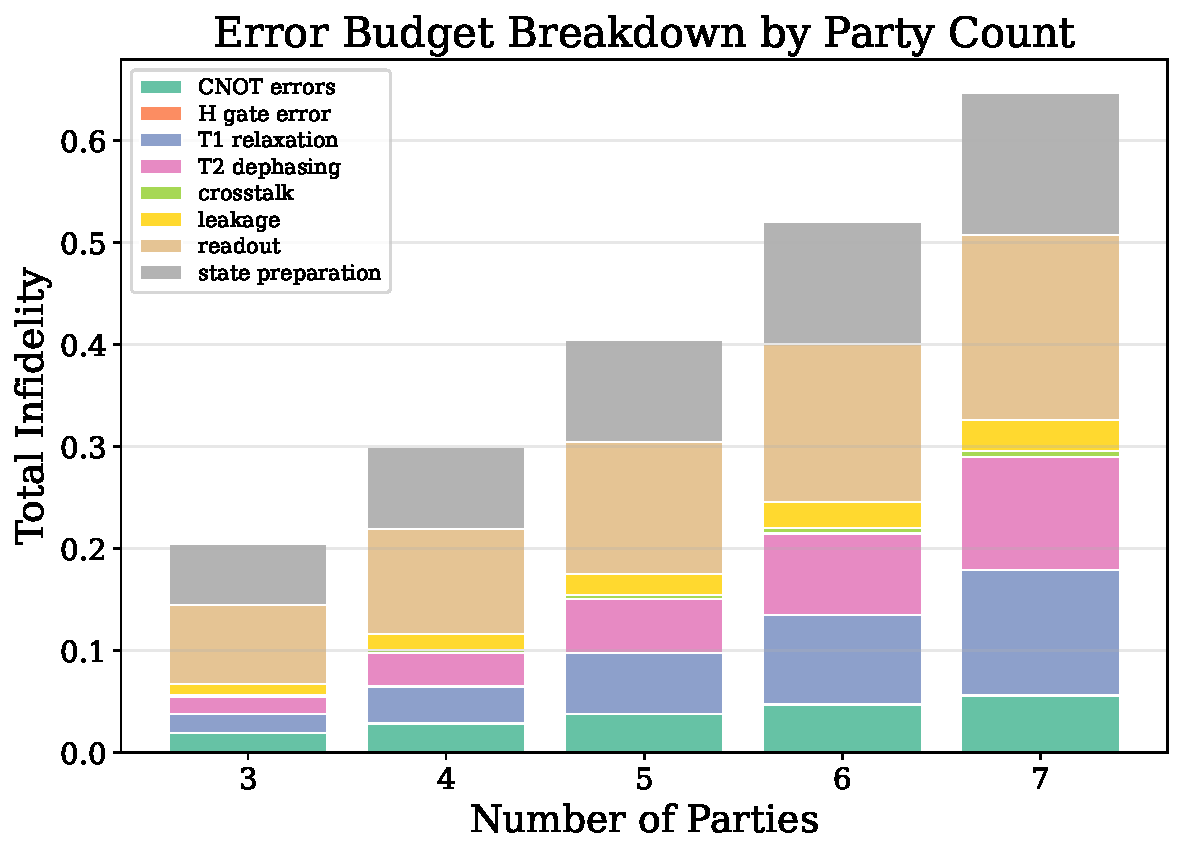
\includegraphics[width=\columnwidth]{figures/fig2_error_budget.pdf}
\caption{Channel-resolved first-order penalty budget for three-qubit GHZ preparation.}
\label{fig:budget}
\end{figure}

\subsection{Secret-sharing performance}
\label{subsec:hbb_results}

\Cref{tab:hbb} summarizes shot-based secret-sharing performance.  The three-party success rate is $89.7\%\pm0.2\%$.  The reported data-basis population is the probability of landing in the two ideal encoded $Z$-basis strings after the secret-bit operation, not the full two-basis GHZ fidelity of \cref{tab:fidelity}.  The $X$-basis QBER increases with $n$, consistent with the higher phase sensitivity of larger GHZ states.  Despite decreasing global fidelity, perfect reconstruction of the three-bit secret occurs in all simulated trials because the majority decoder remains below its effective $50\%$ bit-error threshold.

\begin{table}[H]
\centering
\caption{GHZ secret-sharing benchmark results for $n=3$--$7$ over $100$ trials with $8192$ shots.}
\label{tab:hbb}
\resizebox{\columnwidth}{!}{%
\begin{tabular}{ccccc}
\toprule
$n$ & Success (\%) & Data $P_Z$ & $\qber_X$ & Perfect reconstruction \\
\midrule
3 & $89.7\pm0.2$ & $0.861\pm0.002$ & $0.129\pm0.008$ & 100\% \\
4 & $92.6\pm0.2$ & $0.813\pm0.002$ & $0.164\pm0.009$ & 100\% \\
5 & $91.4\pm0.2$ & $0.761\pm0.003$ & $0.200\pm0.010$ & 100\% \\
6 & $91.3\pm0.2$ & $0.725\pm0.003$ & $0.229\pm0.010$ & 100\% \\
7 & $90.8\pm0.2$ & $0.691\pm0.003$ & $0.253\pm0.012$ & 100\% \\
\bottomrule
\end{tabular}}
\end{table}

\section{Security diagnostics}
\label{sec:security}

\Cref{tab:security} confirms the theoretical prediction of \cref{prop:coherence_suppression} within the two individual-attack stress tests considered here.  Intercept--resend affects both $Z$-basis statistics and $X$-basis coherence.  Entangle--measure leaves $Z$-basis reconstruction almost unchanged but drives $\qber_X$ close to $1/2$.  Thus the $X$-basis check is not a cosmetic addition; it is the observable that diagnoses which-branch information leakage in this benchmark setting.

\begin{table}[H]
\centering
\caption{Diagnostic stress tests of the three-party GHZ secret-sharing benchmark.  Detection uses Eq.~\eqref{eq:detection_rule}.}
\label{tab:security}
\resizebox{\columnwidth}{!}{%
\begin{tabular}{lcccc}
\toprule
Scenario & Success (\%) & $\Delta R_Z$ & $\qber_X$ & Detected \\
\midrule
Honest & $89.7\pm0.4$ & -- & 0.129 & N/A \\
Intercept--resend & $74.6\pm17.6$ & 0.150 & 0.495 & yes \\
Entangle--measure & $89.6\pm0.3$ & 0.000 & 0.485 & yes \\
\bottomrule
\end{tabular}}
\end{table}

A global noise-scale sweep shows operational viability, defined here as success rate above $2/3$, up to $\lambda\approx3.25$.  The GHZ fidelity crosses $2/3$ at approximately $\lambda\approx2.5$, indicating that majority-vote reconstruction can remain operational after the global entanglement witness has substantially degraded.  This sweep is an operational benchmark of reconstruction robustness, not a finite-key security threshold.

\begin{figure}[H]
\centering
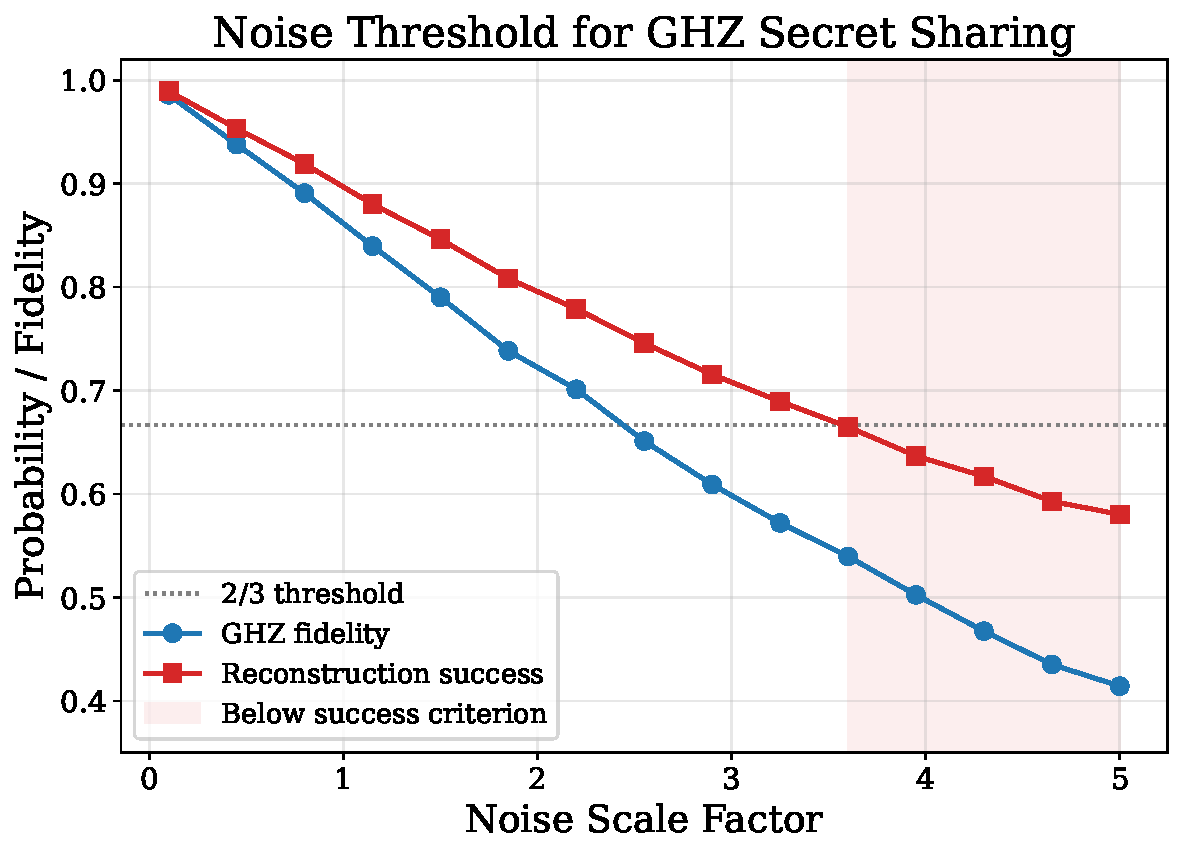
\includegraphics[width=\columnwidth]{figures/fig5_security_threshold.pdf}
\caption{GHZ benchmark fidelity and secret-reconstruction success rate as functions of the global noise scale $\lambda$.}
\label{fig:threshold}
\end{figure}

\section{Hardware validation}
\label{sec:hardware}

\Cref{tab:hardware} compares simulation and hardware estimates on IBM Marrakesh for $n=3,5,7$.  The gaps are $+1.0\%$, $+3.2\%$, and $-0.8\%$, giving an RMS gap of $1.9\%$.  The positive bias at small $n$ is consistent with Marrakesh having longer coherence times than the Falcon-class calibration set.  The sign inversion at $n=7$ is consistent with increased topology- and crosstalk-dependent errors along longer heavy-hex paths.

\begin{table}[H]
\centering
\caption{Hardware validation on IBM Marrakesh.  $\Delta\fid=\fid_{\rm HW}-\fid_{\rm sim}$.}
\label{tab:hardware}
\resizebox{\columnwidth}{!}{%
\begin{tabular}{cccccc}
\toprule
$n$ & $\fid_{\rm HW}$ & $P_Z$ & $C_X$ & $\fid_{\rm sim}$ & $\Delta\fid$ \\
\midrule
3 & 0.961 & 0.967 & 0.955 & 0.951 & +0.010 \\
5 & 0.918 & 0.937 & 0.898 & 0.885 & +0.032 \\
7 & 0.848 & 0.889 & 0.808 & 0.856 & -0.008 \\
\bottomrule
\end{tabular}}
\end{table}

\begin{figure}[H]
\centering
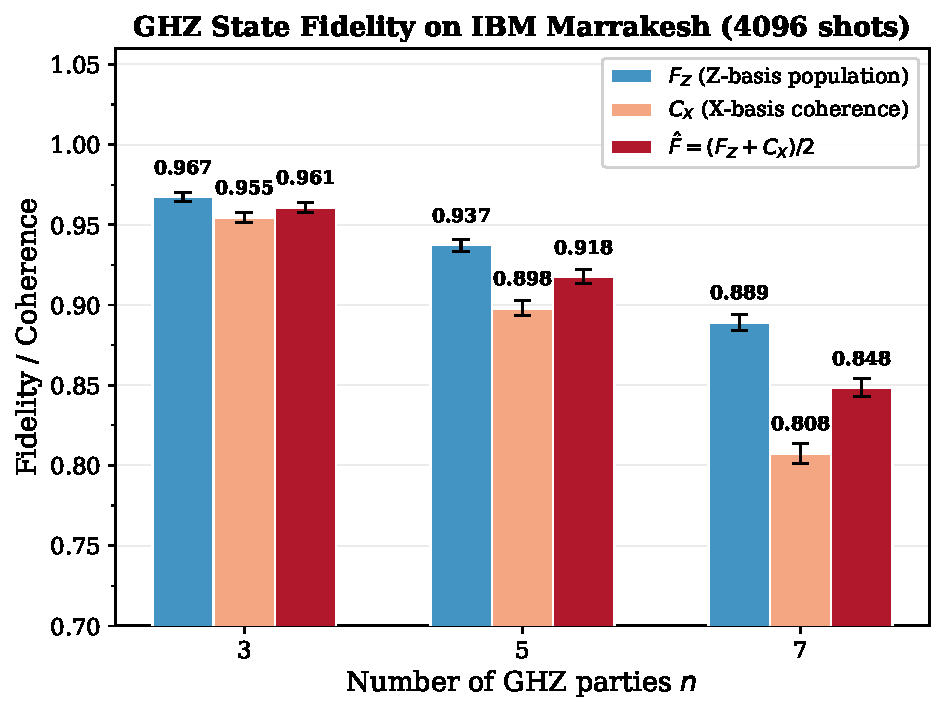
\includegraphics[width=\columnwidth]{figures/fig_hardware_validation.pdf}
\caption{Measured and simulated GHZ fidelity for $n=3,5,7$.}
\label{fig:hardware}
\end{figure}

\section{Discussion}
\label{sec:discussion}

The first implication is methodological.  Reporting only computational-basis populations is insufficient for benchmarking GHZ-based secret sharing because an adversary-like disturbance can preserve $P_Z$ while suppressing $C_X$.  Under the GHZ-support assumption, the two-observable pair $(P_Z,C_X)$ functions simultaneously as a fidelity estimator, an entanglement witness, and an individual-attack diagnostic.

The second implication is hardware-specific.  On short GHZ circuits, SPAM contributes more to the observed infidelity than coherent dynamics or CNOT depolarization.  This does not mean two-qubit gates are unimportant; rather, for this protocol and size range, readout and initialization improvements should deliver the largest immediate performance gains.

The third implication concerns operational figures of merit.  The global GHZ fidelity and the secret-reconstruction probability need not scale identically.  Fidelity is sensitive to global coherence, while reconstruction with majority vote is governed largely by marginal bit errors.  A practical QSS benchmark should therefore report both quantities, not only state fidelity.

Several limitations remain.  The computational-basis data rounds use the operational $X^s$ encoding defined in Eq.~\eqref{eq:decoder}, while a fully device-independent or composably secure HBB implementation would require a separate finite-key treatment of random basis choices, authenticated public discussion, and general coherent attacks.  The leakage channel is treated approximately inside the computational subspace, rather than through explicit qutrit dynamics.  Calibration parameters are treated as static during each simulation campaign, while real superconducting devices drift over hour timescales.  The hardware comparison is cross-architectural and therefore validates physical plausibility rather than a device-specific digital twin.  The attack study covers two canonical individual attacks and should be interpreted as a diagnostic stress test, not as a composable security proof.

\section{Conclusion}
\label{sec:conclusion}

We have developed a theory-guided and hardware-validated benchmark framework for noisy GHZ-based secret sharing.  The analytical contribution is a dual-basis witness showing that computational-basis monitoring alone cannot diagnose population-preserving which-branch disturbances, while $X$-basis coherence directly reveals them.  The numerical contribution is an eight-channel calibrated superconducting-noise simulation of a GHZ secret-sharing benchmark, including fidelity scaling, error budgeting, individual-attack stress tests, and hardware validation.  The results identify SPAM mitigation as the most important near-term hardware target and establish concrete noise margins for GHZ-based reconstruction on present superconducting processors.

\section*{Supplementary Material}
Simulation source code, raw data tables, plotting scripts, hardware-validation metadata, and generated figures are provided in the supplementary repository.

\begin{acknowledgments}
We acknowledge use of IBM Quantum services.  The views expressed are those of the author and do not reflect the official policy or position of IBM or the IBM Quantum team.  We thank the Qiskit development community for the open-source simulation framework.
\end{acknowledgments}

\section*{Author Declarations}

\subsection*{Conflict of Interest}
The author has no conflicts to disclose.

\subsection*{Author Contributions}
Tanvir Hassan: Conceptualization; Methodology; Software; Validation; Formal analysis; Investigation; Data curation; Writing -- original draft; Writing -- review and editing; Visualization.

\subsection*{Ethics Approval}
Ethics approval was not required for this study.

\section*{Data availability}
Simulation source code, device-parameter files, raw CSV data, plotting scripts, and the IBM Quantum hardware-validation job identifier are available in the supplementary repository at \url{https://github.com/tanvir6307/ghz-secret-sharing}.

\appendix

\section{Derivation of the two-observable GHZ fidelity estimator}
\label{app:fidelity_estimator}

Restrict the density matrix to the GHZ support spanned by $\ketzero$ and $\ketone$ plus leakage outside this support.  The fidelity with $\ket{\ghz_n}$ is
\begin{equation}
\fid=\frac{1}{2}\left(\rho_{00,00}+\rho_{11,11}\right)+\mathrm{Re}\,\rho_{00,11}.
\end{equation}
The first term is estimated directly as $P_Z/2$.  The global parity observable satisfies
\begin{equation}
\begin{aligned}
\langle X^{\otimes n}\rangle
&=\rho_{00,11}+\rho_{11,00}\\
&\quad+\mathcal{R}_{\rm comp}.
\end{aligned}
\end{equation}
Here $\mathcal{R}_{\rm comp}$ collects matrix elements coupling complementary bit strings outside the GHZ subspace.  For states whose dominant support remains in the GHZ subspace, these terms are negligible or can be bounded by additional stabilizer measurements.  Therefore $C_X/2$ estimates the off-diagonal contribution, giving Eq.~\eqref{eq:two_observable_fidelity}.

\section{Majority-vote reconstruction bound}
\label{app:majority_bound}

Assume independent helper bit flips with probability $p$.  Reconstruction fails if more than half of the helper outcomes are flipped.  For odd $m=n-1$, the failure probability is
\begin{equation}
P_{\rm fail}(m,p)=\sum_{k=(m+1)/2}^{m}\binom{m}{k}p^k(1-p)^{m-k}.
\end{equation}
Hoeffding's inequality gives
\begin{equation}
P_{\rm fail}(m,p)\leq \exp[-2m(1/2-p)^2],\qquad p<1/2.
\end{equation}
This explains why reconstruction can remain robust even when full-state coherence, and hence GHZ fidelity, has degraded.

\bibliographystyle{aipnum4-2}
\bibliography{references}

\end{document}
